\documentclass{article}


\usepackage{arxiv}

\usepackage[utf8]{inputenc} % allow utf-8 input
\usepackage[T1]{fontenc}    % use 8-bit T1 fonts
\usepackage{hyperref}       % hyperlinks
\usepackage{url}            % simple URL typesetting
\usepackage{booktabs}       % professional-quality tables
\usepackage{amsfonts}       % blackboard math symbols
\usepackage{nicefrac}       % compact symbols for 1/2, etc.
\usepackage{microtype}      % microtypography
\usepackage{lipsum}
\usepackage[numbers, square]{natbib}
\usepackage[inline]{enumitem}

\usepackage{graphicx}
\graphicspath{{./Resources/}}
\usepackage{subcaption}

% for editing
\usepackage{color}


\newcommand{\code}{\texttt}
\newcommand{\edit}{\textcolor{red}}

\title{Predicting Credit Card Default}


\author{
 Group Name: \texttt{Goup N}\\
  Department of Biomechanical Engineering\\
  University College London\\
  London, WC1E 6BT\\
}

\begin{document}
\maketitle

%\begin{abstract}
%\lipsum[1]
%\end{abstract}


% keywords can be removed
%\keywords{First keyword \and Second keyword \and More}


\section{Introduction}

In light of UK Finance expecting the value of credit card payments to rise from £638 billion in 2016 to £942 billion by 2026 \cite{ukfinance}, the problem of credit card delinquency has continued to gain in relevance, not only as a determinant of bank profitability, but also as an important component of broader financial system risk. Reducing damage and uncertainty by identifying counterparty default risk has been shown to be the single most important purpose served by credit risk models utilised by financial institutions \cite{hsu2019enhanced, fatemi2006credit}.


The machine learning use case of gauging credit default risk has been explored at length in literature. Research has primarily gravitated towards analyzing the performance of various statistical models on these data \citep{rosenberg1994quantitative, giudici2001bayesian, lee2002credit, baesens2003benchmarking}. However, other less-explored avenues of investigation exist involving the impact of feature engineering \citep{kamil2014examining, lu2017real, agarwal2010importance} and feature reduction techniques \citep{hu2019feature, mbuvha2019bayesian, piramuthu2004evaluating}. 

We ground our approach to this well-studied problem in what are broadly considered the objectives of machine learning applied to consumer finance: accuracy, interpretability, and efficiency \citep{hand1997statistical}. Our approach falls under the less-explored avenues of feature reduction and behaviour. Specifically, we:
\begin{enumerate*}[label=(\roman*)]
	\item engineer the featuers to extract signal from client behaviour; 
	\item conduct a tripartite feature reduction pipeline to construct three datasets that seek to maximise either interpretability or information;
	\item train a Support Vector Machine Classifier for each reduced dataset; and
	\item construct a final predictor which combines the three models in a voting procedure. 
\end{enumerate*}

\edit{Training performance indicates \dots}. 

%This paper is organized as follows: Section \ref{sec:data_trans} describes the exploration and transformation of the dataset. Section \ref{sec:methodology} outlines the methodology in detail, including feature engineering, feature reduction, and the steps taken to train and evaluate the chosen model. Section \ref{sec:model_training} explains the training and validation process of the model. Section \ref{sec:results} describes the results of the model selection and evaluation procedure, and compares the tripartite voting approach to each individual model's performance. Section \ref{sec:test} presents the trained model's performance on the test set. Finally, Section \ref{sec:conclusion} discusses the findings of the present analysis and suggests avenues for further research in the domain of feature selection.

\section{Data Transformation \& Exploration}
\label{sec:data_trans} 

\subsection{Data Cleaning}

We begin the Data Transformation \& Exploration stage with some simple data cleaning procedures to ensure the data is accurate, reliable and consistent. First, we find a limited number of instances where values with no pre-defined meaning are assigned to \code{MARRIAGE} and \code{EDUCATION}. For \code{MARRIAGE}, we group observations \code{0,3} together under \code{3} (Others) and for \code{EDUCATION}, we group observations \code{4,5,6,0} together under \code{4} (Others).

Secondly, we note that from the perspective of credit card default, small age deviations (e.g. 24 y.o. vs. 26 y.o.) are insignificant. Larger age deviations, however, are important to capture as they can implicitly provide information about income levels, job security and overall financial stability. Therefore, we aim to increase the signal-to-noise ration provided by the \code{AGE} feature by binning it, resulting in a new variable \code{AGE\_BIN}.

Finally, we note that certain features with numerical values are, in fact, categorical. Therefore, we proceed by one-hot encoding \code{AGE, EDUCATION, SEX, MARRIAGE}. Note that we leave \code{PAY\_X} unencoded because it is semi-continuous (i.e. the increase in the figure corresponds to an increase in months outstanding for payment).

\subsection{Target Class Imbalance: Under- and Over-Sampling}

A reasonable assumption for the dataset of credit card defaulters is to assume an imbalance between the defaulters vs. non-defaulters. In order to test this assumption, we plotted the number of clients for each class, as seen in Figure \ref{fig:class_imbalance}. A clear imbalance between the two classes can be observed, with defaulters making up only 22.4\% of the total training instances. 

\begin{figure}[ht]
	\centering
	\begin{subfigure}{.5\textwidth}
		\centering
		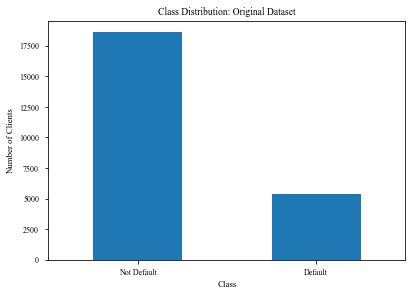
\includegraphics[width=.8\linewidth]{class_imbalance}
		\caption{Imbalanced Classes: Original Dataset}
		\label{fig:class_imbalance}
	\end{subfigure}%
	\begin{subfigure}{.5\textwidth}
		\centering
		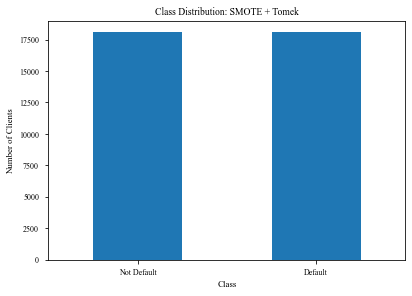
\includegraphics[width=.8\linewidth]{class_balance}
		\caption{Balanced Classes: Post-SMOTE-Tomek}
		\label{fig:class_balance}
	\end{subfigure}
	\label{fig:resampling}
	\caption{Class Resampling}
\end{figure}


Given that the class of non-defaulters is represented by a much larger number of training examples compared to the other class, several inconveniences arise when training classification models on the dataset, as described in \citet{ganganwar2012overview, weiss2004mining}. Broadly speaking, the learning model will provide better accuracy for the majority class due to higher influence of the majority class over the training criteria. Thus, the fact that models are accuracy driven (their goal being to minimise the overall error rate, which is impacted significantly less by the minority class), often leads to the minority class having much lower precision and recall compared to the majority class. Additionally, degenerated models may be produced as the classifiers assume that errors coming from different classes have the same cost.

As a solution to problem, we opt for a data level method of handling imbalance \cite{kotsiantis2006handling}. We deviate from the oversampling approach to the same problem employed by \citet{subasi2019prediction}, who use the Synthetic Minority Over-Sampling Technique (SMOTE) \cite{chawla2002smote}. Driven by results from \citet{batista2004study}, who show that hybrid methods of oversampling and undersampling perform best on a dataset of similar size and class imbalance to ours, we choose the SMOTE + Tomek model. We start by oversampling with SMOTE and further proceed by identifying and removing Tomek links \cite{tomek1976two}. Thus, the class distribution is balanced and better-defined class clusters are created (fig. \ref{fig:class_balance}). For practical purposes we use the implementation presented by \citet{lemaitre2017imbalanced}.

\subsection{Feature Correlation Analysis}
\label{sec:corr_analysis}

To gain further insights into the composition of the dataset, we graphed the \textit{independent} variables of the dataset as a network of nodes positioned along the perimeter of a circle with edges weighted and colored according to the correlation strength, and nodes sized according to each feature's correlation with the target variable. Figures \ref{fig:pos_corr} and \ref{fig:neg_corr} depict the resulting positive and negative correlation graphs, respectively.

%\begin{enumerate}
%	\item To more clearly depict the direction of the pair-wise relationships, separate network graphs were created for positive and negative feature correlations.
%	\item To reflect the magnitude of the pair-wise relationships, edges connecting feature pairs $\left( \mathbf{x}^{(i)}, \mathbf{x}^{(j)} \right)$ were coloured accordingly (with a minimum correlation threshold set at 0.2 for clarity). 
%	\item To underline the independent variables' relationship with the target variable --- which is naturally of great interest --- feature node sizes were made to reflect the magnitude of their relationship with the target.
%\end{enumerate}

\begin{figure}[ht]
	\centering
	\begin{subfigure}{.5\textwidth}
		\centering
		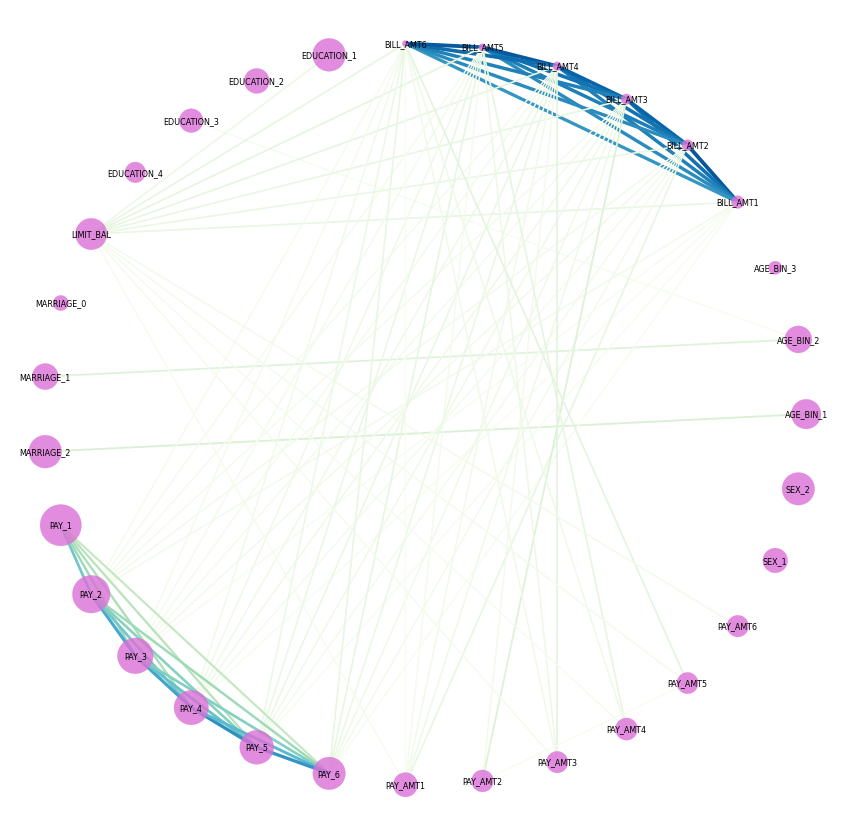
\includegraphics[width=.8\linewidth]{pos_corr}
		\caption{Positive Correlations in Dataset}
		\label{fig:pos_corr}
	\end{subfigure}%
	\begin{subfigure}{.5\textwidth}
		\centering
		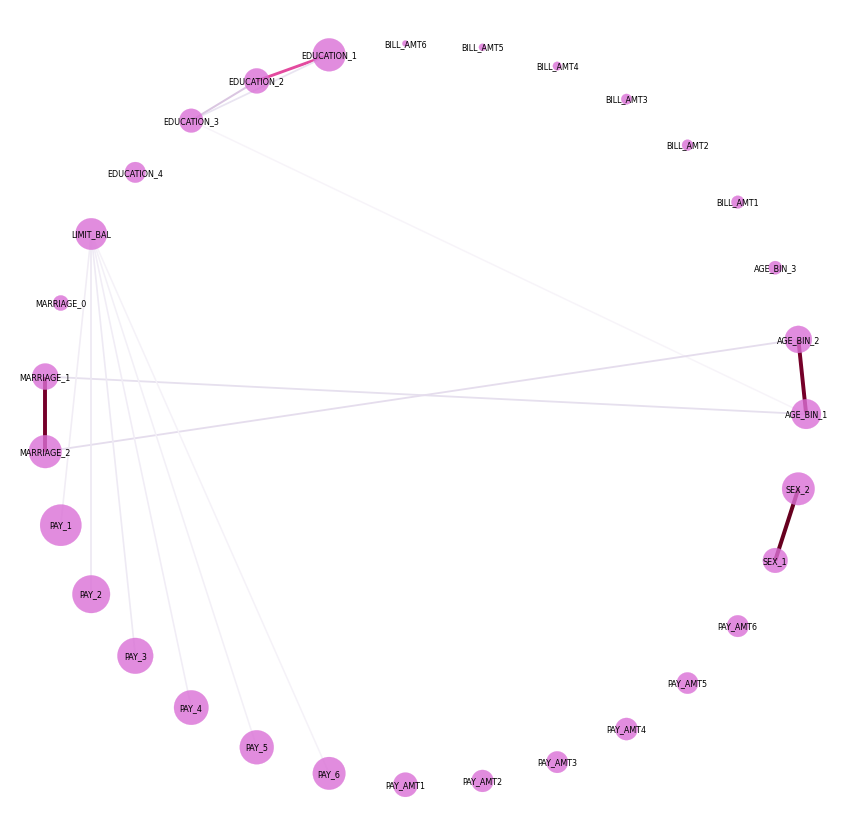
\includegraphics[width=.8\linewidth]{neg_corr}
		\caption{Negative Correlations in Dataset}
		\label{fig:neg_corr}
	\end{subfigure}
	\label{fig:corr}
	\caption{Feature Correlations}
\end{figure}

Interesting insights can be gained from these visualizations. Both graphs clearly display areas of higher correlation densities. Adopting the nomenclature of \citet{hu2019feature}, we refer to these groups of densely-correlated features as `neighbourhoods' in the data. It is evident that the demographic neighbourhoods (\code{EDUCATION}, \code{SEX}, \code{MARRIAGE}, and \code{AGE}) are a simple statistical consequence of the prior one-hot encoding. On the other hand, because \code{PAY} and \code{BILL\_AMT} represent the attribute of a client throughout 6 successive months, the formation of these neighbourhoods can be ascribed to the \textit{sequential time dependency} of the feature groups. Put differently, consider that a client's repayment status and bill amount in May (\code{PAY\_5} and \code{BILL\_AMT5}) are dependent on the client's payment behaviour throughout April, and thus are closely related to the previous months' payment status and bill amount (\code{PAY\_6} and \code{BILL\_AMT6}). Hence, can relevant insights into clients' financial behaviour be extracted by analyzing these neighbourhoods in a time series fashion across the 6 months? This will be examined further in Section \ref{sec:feature_eng}.

\subsection{Target Class Distribution in Most Relevant Features}
\label{sec:target_class_dist}

The prior correlation analysis highlights the importance of the \code{PAY} feature, in terms of both its relationship with other features and its sequential composition and ensuing neighbourhood. What information can be gleaned from it to extract further signals from the data? We divided the dataset into the two target classes, and for each month’s \code{PAY} attribute we visualized the percentage distribution of defaults and non-defaults along each of its possible categorical values.

\begin{figure}[ht]
	\centering
	\begin{subfigure}{.5\textwidth}
		\centering
		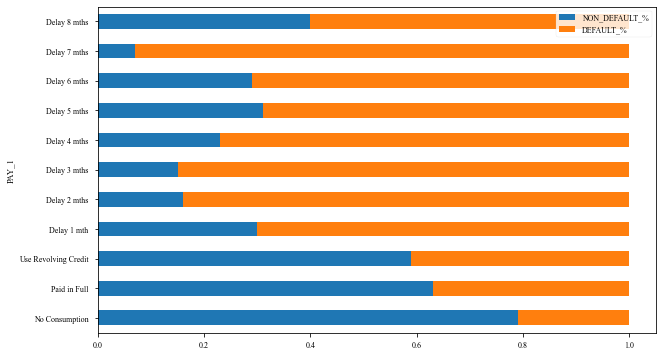
\includegraphics[width=.8\linewidth]{pay_1_dist}
		\caption{\code{PAY\_1} Target Distribution}
		\label{fig:pay_1_dist}
	\end{subfigure}%
	\begin{subfigure}{.5\textwidth}
		\centering
		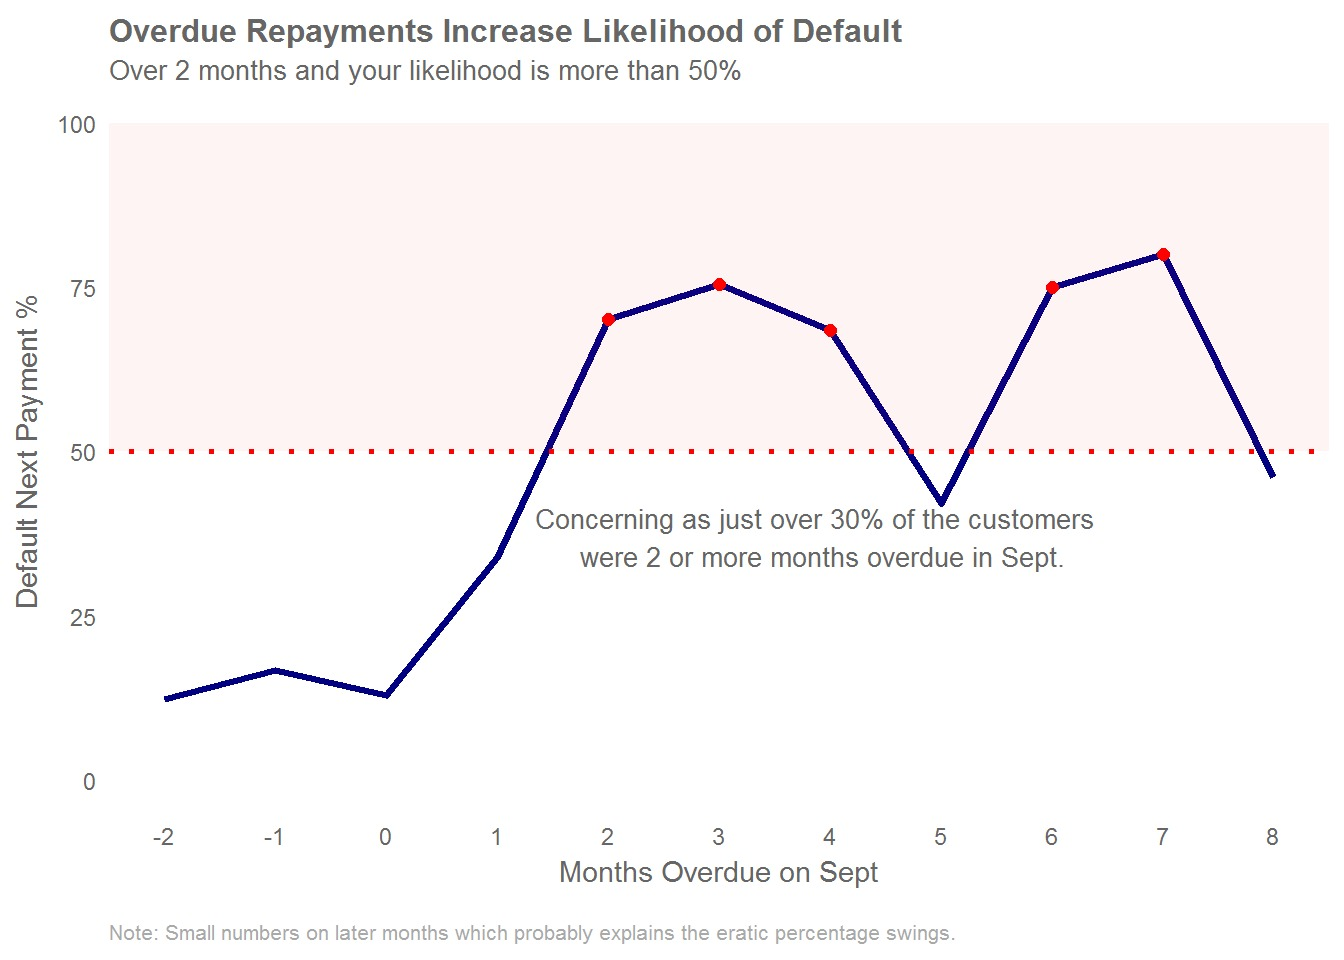
\includegraphics[width=.8\linewidth]{pay_all_dist}
		\caption{Target Distribution Across all \code{PAY} Features}
		\label{fig:pay_all_dist}
	\end{subfigure}
	\caption{\code{PAY} Target Distributions}
	\label{fig:pay_dist}
\end{figure}

As figure \ref{fig:pay_dist} shows, there exist certain clusters of values for which default is less likely. As discussed in the prior correlation analysis, this feature is characterized by its sequential composition. Thus, clustering this behaviour over the 6 months may lead to valuable insights for a financial institution. This will be examined further in the feature engineering.

\section{Methodology Overview}
\label{sec:methodology}

Credit risk modeling has been explored extensively in machine learning literature \citep{mays1998credit}. As is customary in this domain, the lion’s share of research interest has been devoted to testing a wide variety of classifiers (KNNs, Logistic Regression, NNs, SVMs, etc.) to identify best performers \citep{yeh2009comparisons}. \citet{baesens2003benchmarking} find that neural networks and SVMs exhibit the best performance, although simpler methods (LDA, LR) also perform well. A single best performer elusive. On one hand, \citet{huang2004credit} conclude that the difference between SVMs and back-propagation NNs is insignificant. On the other, \citet{li2006evaluation} demonstrate SVM outperformance of NNs, but the size of their dataset disfavours the latter \citep{bellotti2009support}.

Other variants of the research have sought to drive performance through feature engineering to increase predictiveness. \citet{agarwal2010importance} idenfity that features describing client financial behaviour (e.g. FICO scores) exhibit clear correlations with risk of default. \citet{kamil2014examining} examine the impact of financial behaviour \textit{a priori} by evaluating the relationship between clients’ Financial Intelligence Quotient (FiQ) with credit card usage. 

Besides accuracy, efficiency and interpretability are widely considered critical objectives in financial applications of machine learning \citep{hand1997statistical}. Thus, feature reduction has also gathered important attention. Work by \citet{hu2019feature, mbuvha2019bayesian, piramuthu2004evaluating} introduce novel feature selection methods that perform well in credit risk modelling. Because feature selection preserves variable meaning, it protects interpretability \citep{masaeli2010transformation}. Dimensionality reduction approaches like PCA sacrifice interpretability, but have been found to outperform selection approaches \citep{koutanaei2015hybrid}.

Our approach to the present problem furthers work done in the feature engineering and reduction branches of the domain. First, we extract as much behavioural signal as possible from the data in novel ways by emphasising the time dimension of certain features in the dataset. Second, we reduce the dataset to maximise efficiency while protecting accuracy and interpretability in a tripartite fashion: selecting features using best-performing filter methods, selecting features using a simple heuristic, and reducing dimensionality through PCA. Third, we train a SVM Classifier on each of these reduced datasets in a Darwinist process. Fourth, we combine these three models in a final predictor that operates through a tripartite voting of these models.

\subsection{Feature Engineering: Extracting Signal from Client Behaviour Over Time}
\label{sec:feature_eng}

\subsubsection{Feature Creation}

In line with our objective of encoding customer behaviour into the dataset, we engineered a series of features relating to the paying habits of the customers. In total, we added five features which have the general aim of capturing the repayment and billing situation of clients across the entire six month period included in our dataset.

The first 2 variables are looking at averages across the entire time-series. We computed a binary variable called "sufficiency" (\code{SUFF}), which is equal to \code{1} if the average bill amount is less than or equal the average payment amount (i.e. the payments are sufficient to cover the bill amounts over the recorded period) or equal to \code{0} otherwise. Additionally, we computed a simple average of the monthly change in repayment amount (\code{AVG\_PAY\_DELTA}), with the aim of recording the payment trend for a particular consumer. Here, a positive average MoM change in payment amount should be indicative of a solid financial situation for the client and we expect a negative correlation with the probability of default.

Then, we take inspiration from XX and create 3 "frequency" variables, motivated by the desire to record the number of occurrences of very favourable / unfavourable credit events during the six months included in the dataset. \code{PAY\_DELAY\_FREQ} stores the number of instances the customer was behind on payment for more than 3 months. \code{PAY\_TIMELY\_FREQ} is computed in similar fashion, but this time for the number of instances the client is on time with payment. Both features are created based on the \code{PAY\_X} variables included in the original dataset. Finally, \code{REPAY\_FREQ} is another "frequency" variables, this time computed based on the \code{PAY\_AMTX} variables included in the original dataset. It stores the number of instances when the customer executed repayments (\code{PAY\_AMTX} > 0). While we expect \code{PAY\_TIMELY\_FREQ} \& \code{REPAY\_FREQ} to be negatively correlated with the default probability and indicative of a solid customer profile, a high value for \code{PAY\_DELAY\_FREQ} is expected to be a predictor of default and a reflection of sub-optimal customer paying behaviour from the bank's perspective.

\subsubsection{Clustering Latitudinal Client Behaviour by Time-Based Features}

As noted in the exploration of the dataset’s features in Sections \ref{sec:corr_analysis} and \ref{sec:target_class_dist}, there exist motivations to further explore the characteristics of certain independent variables whose correlation densities formed neighbhourhoods in the data: \code{PAY} and \code{BILL\_AMT}. Because our emphasis on characterising client behaviour implies a focus on their agency, we considered the examination of \code{PAY} and \code{BILL\_AMT} to be dissimilar. While the former proxies for a client’s repayment behaviour, the latter merely represents what the client \textit{should} pay, not what they \textit{did} pay. Thus, it made sense in the context of our analysis to instead consider \code{PAY\_AMT}. Because each of these payment amounts are correlated with each of the \code{BILL\_AMT} features, as exemplified in fig. \ref{fig:pos_corr}, this `change of variable` is justified for our investigative purposes.


How should this behaviour be characterised? Following our analysis of the different `clusters’ of defaulters and non-defaulters apparent in the distribution of the \code{PAY} variable, we chose to try to identify trends in client repayment behaviour by finding clusters in these features across the 6 months spanned by the dataset. To do so, we considered client records for each feature along the six months as data points in a six-dimensional feature space. Note that due to the characterization of these variables, proximity between these points can be measured as their distance in Euclidean terms\footnote{\code{PAY\_AMT} is continuous, and thus suitable for this metric. While \code{PAY} is discrete, it also contains values along the reals, since the range represents increasing repayment delay. Thus, it is also suitable.} Hence, we approached this clustering task using the popular K-Means algorithm. 

%While we recognize that this algorithm is sensitive to changes in data, we note that this dataset is static. Furthermore, the proposed algorithm is not intended to be trained and deployed in an online learning fashion. Thus, employing K-Means is satisfactory for the task at hand. 

A K-Means model was trained on a range of 3 - 7 clusters for both variables. This reduced range was chosen deliberately with the aim of increasing the interpretability of results, which is important in the context of our use case. We identified the optimal number of clusters as $k = 3$ for both features using the Average Silhouette Method \citep{rousseeuw1987silhouettes}. After training a K-Means model with 3 clusters on each feature group, we plotted the centroids of each cluster to reflect the groups of prototypical customer behaviours (see fig. \ref{fig:time_clusters}).

\begin{figure}[ht]
	\centering
	\begin{subfigure}{.5\textwidth}
		\centering
		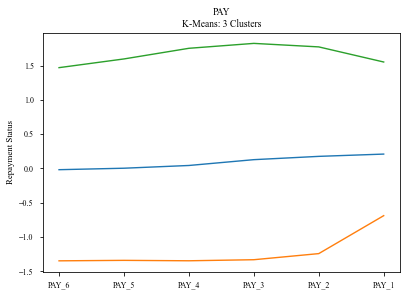
\includegraphics[width=.8\linewidth]{pay_clusters}
		\caption{Clusters for \code{PAY}}
		\label{fig:time_clusters_pay}
	\end{subfigure}%
	\begin{subfigure}{.5\textwidth}
		\centering
		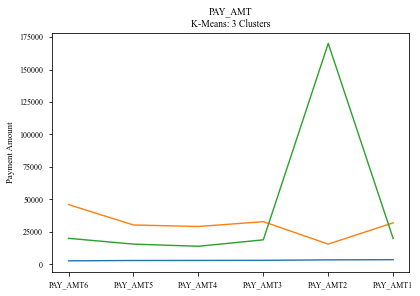
\includegraphics[width=.8\linewidth]{pay_amt_clusters}
		\caption{Clusters for \code{PAY\_AMT}}
		\label{fig:time_clusters_pay_amt}
	\end{subfigure}
	\caption{Time-Based Feature Clusters}
	\label{fig:time_clusters}
\end{figure}

The graphs reveal interesting insights into the behaviour of the bank's clients. Repayment statuses display three clear variants. Clients that are generally behind in payments (higher risk of default); clients that use revolving credit on a recurrent basis (i.e. pay the minimum amount per month) (less risk of default); and clients that either do not consume or pay in full (least risk of default). Similarly, payment amounts reveal three characteristic schedules. Clients that pay near zero amounts across the 6 months (probably corresponding to those who do not consume); clients that pay regularly across the 6 months; and clients that pay large amounts towards the end of the period. 

To enrich the data with these analyses, cluster allocations were encoded in the dataset in the form of two new features, \code{PAY\_CLUSTER} and \code{PAY\_AMT\_CLUSTER}. 

\subsection{Feature Reduction: Feature Selection \& Dimensionality Reduction}

\subsubsection{Feature Selection: Network Structure-based Feature Selection Algorithm (NSFSA)}

The first feature selection methodology we adopted was motivated by the objective of selecting the most relevant variables in the data while preserving the dataset's underlying structure. To do so, we follow the approach devised by \citet{hu2019feature}, dubbed Network Structure-based Feature Selection Algorithm (NSFSA). The goal of the algorithm is to select the best subset of features in the data that removes data redundancy while preserving an underlying network structure.

%\begin{enumerate}
%	\item A network structure is identified in the dataset, whereby features are grouped into neighbourhoods characterised by representative characteristics. 
%	\item For each feature, a proxy of its relevance in the neighourhood is computed as the sum of its correlations with all other features in that group. This sum is then multiplied by the feature's correlation with the target variable, to account for this important relationship.
%%	\begin{equation}
%%		w_{\mathbf{x}^{(i)}} = \rho_{\mathbf{x}^{(i)}, y^{(i)}} \left(\sum_{x^{(j)} \in N_{\mathbf{x}^{(i)}}} |\rho_{\mathbf{x}^{(i)}, \mathbf{x}^{(j)}} | \right)
%%	\end{equation}
%%	where $N_{\mathbf{x}^{(i)}}$ represents the set of features belonging to $\mathbf{x}^{(i)}$'s neighbourhood.
%	\item The features in each neighbourhood are ranked according to this computed metric. To eliminate redundancy, only the top $n$ features of each neighbourhood are selected to form the subset of the dataset.
%\end{enumerate}

As the first step of NSFSA, we sought a principled approach towards organising the data's features into a coherent network structure. We present a novel methodology for this purpose. Given the different scales and units of the data's features and the varied categorical and numeric types, a typical distance-based clustering algorithm would not be suitable. An alternative course of action was motivated by the correlation graph presented in Section \ref{sec:corr_analysis}, where neighbourhoods of features are formed by areas of higher correlation densities. Thus, we attempted to use correlation as a proxy for the proximity between feature and defined a proximity metric, $p_{\mathbf{x}^{(i)}, \mathbf{x}^{(j)}}$, as:
\begin{equation}
	p_{\mathbf{x}^{(i)}, \mathbf{x}^{(j)}} = \frac{1}{|\rho_{\mathbf{x}^{(i)}, \mathbf{x}^{(j)}}| + \epsilon} -1 
\end{equation}
where $\epsilon \simeq 0$ to ensure validity for uncorrelated features, and 1 is subtracted such that the distance for perfectly correlated features is 0. Thus, highly-correlated features result in a smaller metric than uncorrelated ones.

We adopt an Agglomerative Clustering model due to its greater flexibility and higher quality tree structure \citep{walter2008fast}. Despite these advantages, this model requires the preemptive specification of the desired number of clusters. To select this, we follow the Thorndike method, a popular heuristic approach in machine learning literature involvig dendrogram analysis to determine the optimal groups in a hierarchy \citep{thorndike1953belongs}. This procedure reveals 5 clusters are optimal for our data (see fig. \ref{fig:dendrogram}). Because we seek to form neighbourhoods out of densely-correlated features, we trained an Agglomerative Clustering algorithm to form 5 clusters based on the single linkage method. Similarly, the single linkage method was desirable given it results in clusters in which elements in the cluster are more similar to at least one other neighbour than to external elements \citep{el1989comparison}. The resulting network structure can be visualized in fig. \ref{fig:nbr_graph}.

\begin{figure}[ht]
	\centering
	\begin{subfigure}{.5\textwidth}
		\centering
		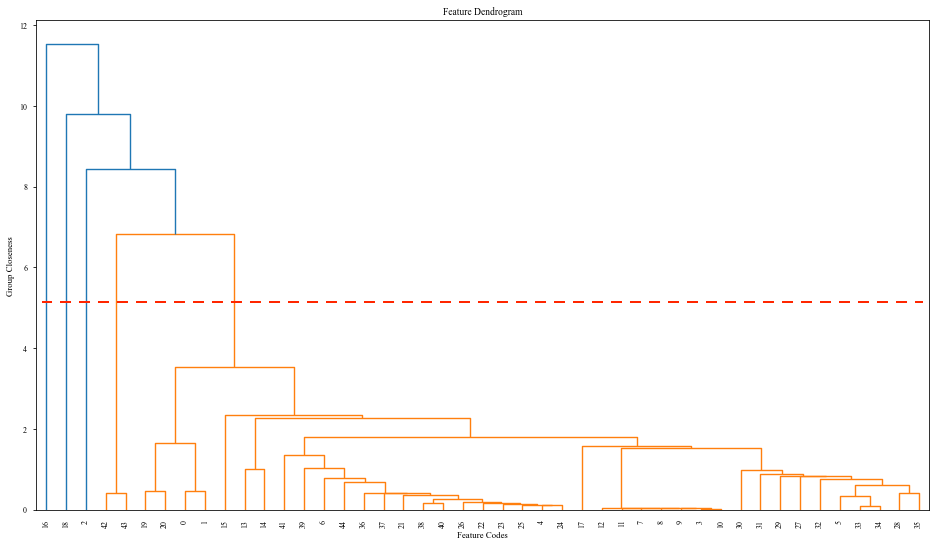
\includegraphics[width=.8\linewidth]{dendrogram}
		\caption{Feature Dendrogram: Thorndike Method}
		\label{fig:dendrogram}
	\end{subfigure}%
	\begin{subfigure}{.5\textwidth}
		\centering
		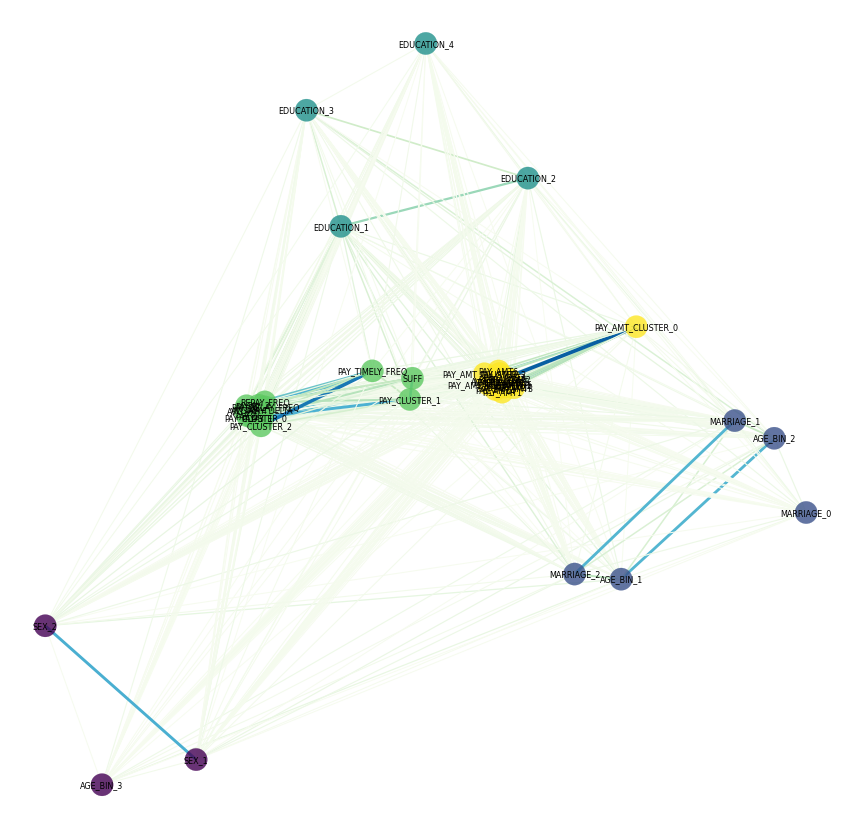
\includegraphics[scale=0.25]{nbr_graph}
		\caption{Neighbourhood Structure}
		\label{fig:nbr_graph}
	\end{subfigure}
	\caption{Network Structure Analysis}
	\label{fig:nbr_structure}
\end{figure}
%This network structure makes contextual sense and displays clear characteristics. First, the demographic and monetary features are clearly separated. These demographic neighbourhoods are largely intuitive: the \code{EDUCATION} variables are all grouped together, and \code{AGE}, \code{MARRIAGE}, and \code{SEX} form two neighbourhoods. On the other hand, monetary features are separated in groups of discrete and continuous values. 
Second, for each feature, a proxy of its relevance in the neighourhood was computed as the sum of its correlations with all other features in that group, multiplied by the feature's correlation with the target variable.

The final step of NSFSA involves ranking the features in each neighbourhood according to the previous metric, and selecting the top $n$ of each neighbourhood to form the best subse that retains the network structure. We chose the top two. Although a higher number of top features would increase the variance of the data, a smaller number of features is desirable for our analysis because it increases interpretability. 

\subsubsection{Feature Selection: Network-Based Heuristic}

Driven by the overarching aim of reducing dimensionality and maximising interpretability, we motivated a simpler `heuristic' feature selection method as seeking to not only summarise the set of features in the dataset but also the dataset's structure itself, thereby narrowing the focus into a single neighbourhood of features. From a use case standpoint, this approach is compelling: if a financial institution can zero in on a set of features with similar characteristics that can best predict credit risk, it may streamline its processes and enhance interpretability. 

In this case, we segregate feature correlations with the target variable as the sole metric of interest. This is because a higher correlation of the overall feature subset with the target variable should lead to greater signal. To do so,  we employed the network structure devised in the previous section. Then, for each neighbourhood, we omputed the sum of the features' correlation with the target variable. The neighbourhood with the highest computed metric was selected as the best subset of features. 

\subsubsection{Dimensionality Reduction: PCA}

The motivation behind our third and final feature reduction methodology is to capture the information provided by the entire original feature set through a computationally smaller subset. More specifically, we are aiming to extract the most important information from our enhanced feature space and compress its size by only going forward with this important information. For this purpose we choose one of the oldest and most widely used multivariate statistical techniques, Principal Component Analysis (PCA) \cite{abdi2010principal}.

The procedure for computing the principal components in the basic version of PCA (used here) is fairly straightforward \cite{jolliffe2016principal}. After the data is standardised, the sample covariance matrix is computed for the original dataset. Then, the eigenvectors and associated eigenvalues are computed for the sample covariance matrix. These eigenvectors are sorted in decreasing order of their corresponding eigenvalues. The principal components are the linear combinations of the original matrix and the eigenvectors (obtained as described below).

The results of our analysis can be observed in Figure \ref{fig:pca_results}. In order to select the number of components to be kept after the PCA step, we plot the cumulative proportion of variance explained for all principal components (scree plot). After setting our target at 95\% of explained variance, the resulting feature subset contains 25 components.
\begin{figure}[ht]
	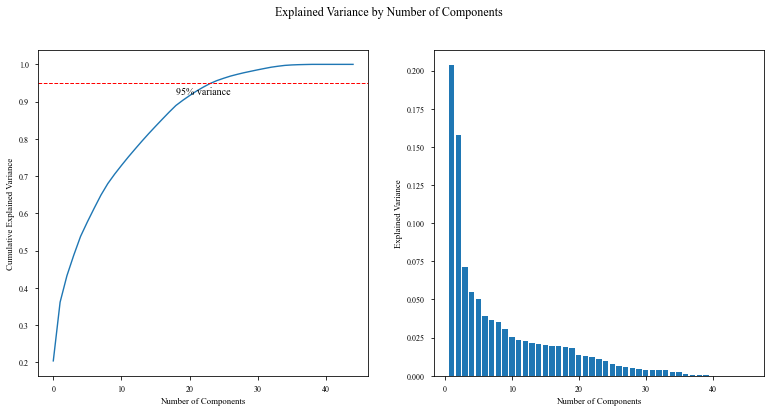
\includegraphics[scale=0.4]{PCA}
	\centering
	\caption{PCA Results}
	\label{fig:pca_results}
\end{figure}

\subsection{Model Selection, Training, \& Validation}

\section{Model Training \& Validation}
\label{sec:model_training}

\section{Results}
\label{sec:results}

\section{Final Predictions on Test Set}
\label{sec:test}

\section{Conclusion}
\label{sec:conclusion}

\bibliographystyle{abbrvnat} 
\bibliography{bib}  %%% Remove comment to use the external .bib file (using bibtex).
%%% and comment out the ``thebibliography'' section.

\end{document}